%%%%%%%%%%%%%%%%%%%%%%%%%%%%%%%%%%%%%%%%%%%%%%%%%%%
%% LaTeX book template                           %%
%% Author:  Amber Jain (http://amberj.devio.us/) %%
%% License: ISC license                          %%
%%%%%%%%%%%%%%%%%%%%%%%%%%%%%%%%%%%%%%%%%%%%%%%%%%%

\documentclass[11pt, fleqn]{book}
\usepackage[b5paper, top=2.5cm, bottom=2.5cm, left=2cm, right=2cm]{geometry} %para personalizar el tamaño y margenes de la hoja
\usepackage[T1]{fontenc}
\usepackage[utf8]{inputenc}
\usepackage{lmodern}
%%%%%%%%%%%%%%%%%%%%%%%%%%%%%%%%%%%%%%%%%%%%%%%%%%%%%%%%%
% Source: http://en.wikibooks.org/wiki/LaTeX/Hyperlinks %
%%%%%%%%%%%%%%%%%%%%%%%%%%%%%%%%%%%%%%%%%%%%%%%%%%%%%%%%%
\usepackage[colorlinks=false]{hyperref}
\usepackage{graphicx}
\usepackage[spanish, es-noshorthands]{babel}

\usepackage{float} %lo agregue para las tablas qeu andaban de rebeldes
\usepackage{amsmath} %lo agregue para la numeración de las Ecuaciones
\usepackage{amsthm}
\usepackage{amsfonts}
\usepackage{mathtools}
\usepackage{amssymb}
\usepackage{stackengine}
\usepackage{graphicx} %para las imagenes
\usepackage{float}
%*************Aun falta el graphics path%
\usepackage{lscape} %necesario para usar la propiedad "begin{landscape}"
\usepackage{longtable} %necesario para usa la propiedad "longtable"
\usepackage{booktabs} %necesario para usar la propiedad "toprule"
\usepackage{mathrsfs}

%%%%%%%%%%%%%%%%%%%%%%%%%%%%%%%%%%%%%%%%%%%%%%%%%%%%%%%%%%%%%%%%%%%%%%%%%%%%%%%%
% 'dedication' environment: To add a dedication paragraph at the start of book %
% Source: http://www.tug.org/pipermail/texhax/2010-June/015184.html            %
%%%%%%%%%%%%%%%%%%%%%%%%%%%%%%%%%%%%%%%%%%%%%%%%%%%%%%%%%%%%%%%%%%%%%%%%%%%%%%%%
% You might want to add short description about each chapter in this book.
%The website\footnote{\url{https://github.com/amberj/latex-book-template}} for this file contains:

\newenvironment{dedication}
{
   \cleardoublepage
   \thispagestyle{empty}
   \vspace*{\stretch{1}}
   \hfill\begin{minipage}[t]{0.66\textwidth}
   \raggedright
}
{
   \end{minipage}
   \vspace*{\stretch{3}}
   \clearpage
}

%%%%%%%%%%%%%%%%%%%%%%%%%%%%%%%%%%%%%%%%%%%%%%%%
% Chapter quote at the start of chapter        %
% Source: http://tex.stackexchange.com/a/53380 %
%%%%%%%%%%%%%%%%%%%%%%%%%%%%%%%%%%%%%%%%%%%%%%%%
%%%%%%%%%%%%%%%%%%%%%%%%%%%%%%%%%%%%
% Give credit where credit is due. %
% Say thanks!                      %
%%%%%%%%%%%%%%%%%%%%%%%%%%%%%%%%%%%%

\makeatletter
\renewcommand{\@chapapp}{}% Not necessary...
\newenvironment{chapquote}[2][2em]
  {\setlength{\@tempdima}{#1}%
   \def\chapquote@author{#2}%
   \parshape 1 \@tempdima \dimexpr\textwidth-2\@tempdima\relax%
   \itshape}
  {\par\normalfont\hfill--\ \chapquote@author\hspace*{\@tempdima}\par\bigskip}
\makeatother

%%%%%%%%%%%%%%%%%%%%%%%%%%%%%%%%%%%%%%%%%%%%%%%%%%%
% First page of book which contains 'stuff' like: %
%  - Book title, subtitle                         %
%  - Book author name                             %
%%%%%%%%%%%%%%%%%%%%%%%%%%%%%%%%%%%%%%%%%%%%%%%%%%%

% Book's title and subtitle
\title{\Huge {Transferencia de masa} }
% Author
\author{\textsc{Octavio Manero Brito}}

\begin{document}

\frontmatter
\maketitle

%%%%%%%%%%%%%%%%%%%%%%%%%%%%%%%%%%%%%%%%%%%%%%%%%%%%%%%%%%%%%%%
% Add a dedication paragraph to dedicate your book to someone %
%%%%%%%%%%%%%%%%%%%%%%%%%%%%%%%%%%%%%%%%%%%%%%%%%%%%%%%%%%%%%%%
\begin{dedication}
Dedicated to Calvin and Hobbes.
\end{dedication}

%%%%%%%%%%%%%%%%%%%%%%%%%%%%%%%%%%%%%%%%%%%%%%%%%%%%%%%%%%%%%%%%%%%%%%%%
% Auto-generated table of contents, list of figures and list of tables %
%%%%%%%%%%%%%%%%%%%%%%%%%%%%%%%%%%%%%%%%%%%%%%%%%%%%%%%%%%%%%%%%%%%%%%%%

\tableofcontents
%\listoffigures
%\listoftables

\mainmatter
%%%%%%%%%%%
% Preface %
%%%%%%%%%%%
\chapter*{Prefacio}


%%%%%%%%%%%%%%%%
% NEW CHAPTER! %
%%%%%%%%%%%%%%%%
\chapter{Capitulo 1}
\section{Lo de los chavalos XD}
AQUÍ va todo lo anterior 
%\section*{esto es una sección}
%\subsection{esto es una subsección}
%\subsubsection{esto es una subsubsección}
%\begin{itemize}
%\item mi primer item 
%\item mi seguendo item
%\end{itemize}
%\begin{itemize}
 %  \item[1.-] mi primer item 
%\item[b.] mi seguendo item
%  \end{itemize}
%\begin{enumerate}
%  \item punto 1
%  \item punto 2
%  \item punto 3
%\end{enumerate}

  

\section{Difusión con reacción química homogénea}

\begin{minipage}{0.5\textwidth} 
    \centering
    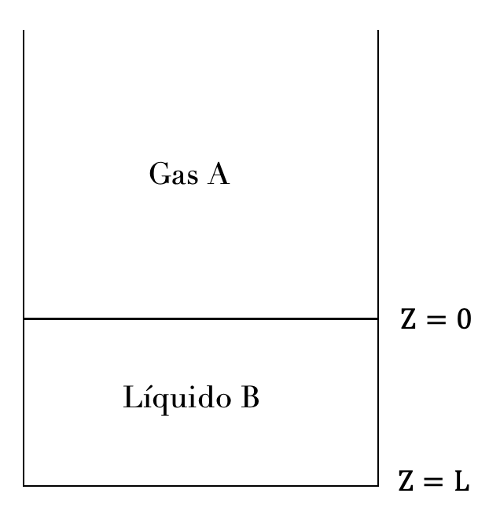
\includegraphics[width=0.8\linewidth]{Capitulo2/Imagenes/Fig_2.9.png} 
    \captionof{figure}{Absorción de A en B con reacción homogénea en la fase líquida} 
    \label{fig:Fig_2.9}
\end{minipage}%
\begin{minipage}{0.4\textwidth} 
    En la figura \textbf{\eqref{fig:Fig_2.9}}, el gas \( A \) se disuelve en el líquido \( B \). Al difundirse \( A \) en \( B \), ocurre una reacción \( A + B \xrightarrow{} AB \). Por ejemplo, la absorción de \( CO_2 \) en una solución de NaOH.
        En este caso, el proceso es descrito por la ecuación \textbf{\eqref{eq_1.30}}, en la cual, no hay dependencia con el tiempo y el sistema está en reposo \( \underline{v} = 0 \).
\end{minipage}
    

\vspace{1 cm}
Suponiendo una reacción de primer orden para la descomposición de A, la ecuación \textbf{\eqref{eq_1.30}} se reduce a:

\begin{equation}   
 \mathscr{D}_{AB}\frac{d^2(C_A)}{dz^2}+R_A=0
 \label{eq_2.55}
\end{equation}


En donde:\begin{equation}
    R_A=\frac{d(C_A)}{dt}=-kC_A
    \label{eq_2.56}
\end{equation}
Este sistema otorga las siguientes condiciones de frontera:

\begin{equation}
    C_A|_{z=0} = C_{A0}, \quad \frac{d(C_A)}{dz}\bigg|_{z=L} = N_{Az}|_{z=L} = 0
    \label{eq_2.57}
\end{equation}

Se definen las siguientes variables adimensionales: $\Gamma=\frac{C_A}{C_{A0}}$ y $\zeta=\frac{z}{L}$

La ecuación \eqref{eq_2.55} se transforma en:
\begin{equation}
    \frac{d^2\Gamma}{d\zeta^2}-\left(\frac{k_1L^2}{\mathscr{D}_{AB}}\right)\Gamma=0
    \label{eq_2.58}
\end{equation}
\quad donde
\begin{equation}
  \phi=\left( \frac{k_1L^2}{\mathscr{D}_{AB}}\right)^{1/2}
\end{equation}

es el módulo de Thiele. \\Las condiciones de frontera adimensionales son ahora:
\begin{equation}
 \Gamma|_{\zeta=0}=1   
\quad \text{y} \quad
 \frac{d\Gamma}{d\zeta}|_{\zeta=1}=0   
 \label{eq_2.60}
\end{equation}

La solución de la ecuación \eqref{eq_2.58} corresponde a:
\begin{equation}
    \Gamma=C_1\cosh({\phi\zeta})+C_2\sinh({\phi\zeta})
    \label{eq_2.61}
\end{equation}
Aplicando \eqref{eq_2.61} obtenemos $C_1$ y $C_2$:

 $C_1=1$ y $0=\phi \sinh({\phi})+C_2\phi \cosh(\phi)\longrightarrow C_2=-\frac{\sinh(\phi)}{\cosh({\phi})}=-\tanh({\phi})$
La ec. \eqref{eq_2.60} tiene la siguiente solución particular:
 \begin{equation}
  \Gamma=\frac{\cosh[{\phi(1-\zeta)}]}{\cosh({\phi})}   
  \label{eq_2.62}
 \end{equation}

La concentración promedio de A en la fase líquida es;

 \begin{equation}
     \overline{\Gamma}=\frac{\int_0^1\Gamma d\zeta}{\int_0^1d\zeta}=\frac{1}{\cosh(\phi)}\left[\frac{\sinh[\phi(1-\zeta)]_{0}^1}{-\phi}\right]=\frac{\tanh(\phi)}{\phi}
     \label{eq_2.63}
 \end{equation}
 
El flux molar en $z=0$ es:

\begin{equation}
    N_{Az}|_{z=0}=-\mathscr{D}_{AB}\frac{d(C_A)}{dz}|_{z=0}=-\mathscr{D}_{AB}\frac{C_{A0}}{L}\frac{d\Gamma}{d\zeta}|_{\zeta=0}=\mathscr{D}_{AB}\frac{C_{A0}}{L}\phi\tanh(\phi)
\end{equation}



\subsection{Absorción de gas con reacción química en un tanque de agitación}
Considere un sistema en el que el gas A disuelto se combina con el líquido B por una reacción química de primer orden. Por ejemplo, la absorsión de $SO_2$ o $H_2S$ en NaOH en solución acuosa.

\begin{figure}[H]
    \centering
    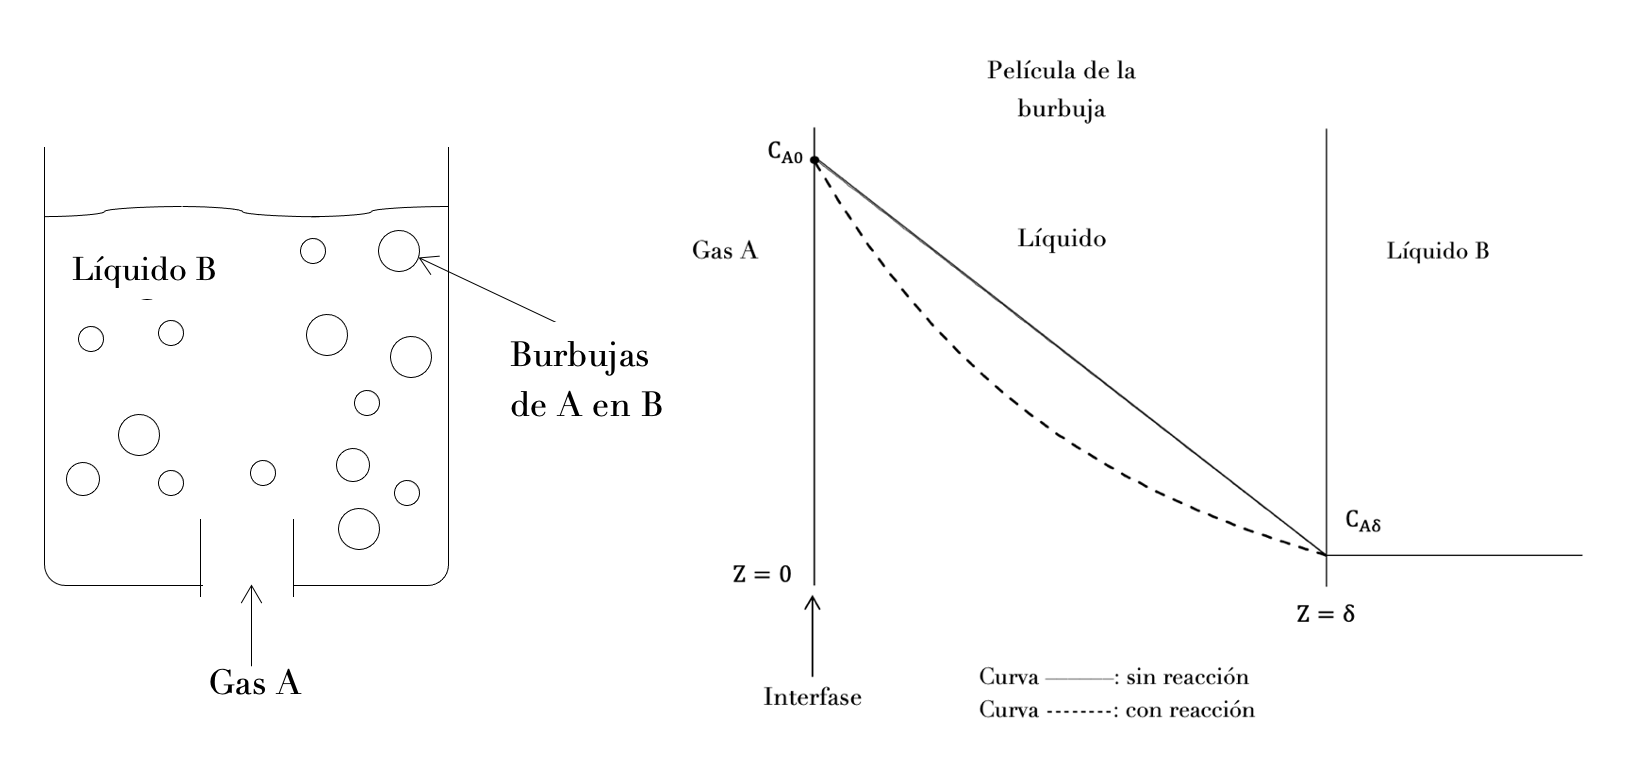
\includegraphics[width=\linewidth]{Capitulo2/Imagenes/Fig_2.10.png}
    \caption{Perfil de concentración predicho en la película de líquido que rodea a una burbuja}
    \label{fig:fig_2.10}
\end{figure}

Condiciones de forntera:
\begin{equation}
    C_A|_{z=0}=C_{A0} \quad\text{y}\quad
    C_A|_{z=\delta}=C_{A\delta}
\end{equation}
O en variables adimensionales:
\begin{equation}
    \Gamma|_{\zeta=0}=1 \quad \text{y} \quad
    \Gamma|_{\zeta=1}=B
        \label{eq_2.66}
\end{equation}
En donde 
\begin{equation*}
    \zeta = \frac{z}{\delta}, \quad \Gamma = \frac{C_A}{C_{A0}}, \quad B = \frac{C_{A\delta}}{C_{A0}}, \quad \phi^2 = \frac{k_1 \delta^2}{\mathscr{D}_{AB}}
\end{equation*}


La ecuación \eqref{eq_2.61} con las condiciones \eqref{eq_2.66} tiene la siguiente solución:

\begin{equation}
    \Gamma=\frac{\sinh(\phi)\cosh(\phi\zeta)+(B-\cosh(\phi))\sinh(\phi\zeta)}{\sinh(\phi)}
    \label{eq_2.67}
\end{equation}
La ecuación \eqref{eq_2.67} describe el perfil de la curva con reacción. Se supone que la concentración de A fuera de la película es $C_{A\delta}$, por lo que, si la superficie de todas las burbujas en la superficie es S, la cantidad de A consumida por la reacción química es:

\begin{equation}
    SN_{Az}|_{z=\delta}=-S\mathscr{D}_{AB}\frac{dC_A}{dz}|_{z=\delta}=Vk_1C_A\delta
    \label{eq_2.68}
\end{equation}
En donde V es el volumen de la fase líquida.
Luego:

\begin{equation*}
    -\frac{dC_A}{dz}|_{z=\delta}=-\frac{C_{A0}}{\delta}\frac{d\Gamma}{d\zeta}|_{\zeta=1}=\frac{Vk_1C_{A\delta}}{S\mathscr{D}_{AB}}\longrightarrow-\frac{d\Gamma}{d\zeta}|_{\zeta=1}=\frac{V}{S\delta}\phi^2B
\end{equation*}
Como $\cosh^2(\phi)-\sinh^2(\phi)=1$, de la ec. \eqref{eq_2.67} se obtiene:

\begin{equation*}
    \frac{B\cosh(\phi)-1}{\sinh(\phi)}=-\frac{V}{S\delta}B\phi\longrightarrow B(\cosh(\phi)+\frac{V}{S\delta}\phi\sinh(\phi))=1
\end{equation*}
Substituyendo B en la solución para Gamma \eqref{eq_2.67}, obtenemos:
\begin{equation}
    \Gamma=\frac{\cosh(\phi)\cosh(\phi\zeta)-\cosh(\phi)\sinh(\phi\zeta)}{\sinh(\phi)}+\frac{\sinh(\phi)\zeta}{\sinh(\phi)}[\frac{1}{\cosh(\phi)+\frac{V\phi\sinh(\phi)}{S\delta}}]
    \label{eq_2.69}
\end{equation}
El flux de masa absorbido con reacción química ( normalizada) es:

\begin{equation}
\begin{split}
    \widetilde{N} &= \frac{N_{Az}}{\mathscr{D}_{AB}\frac{C_{A0}}{\delta}} = -\frac{\mathscr{D}_{AB}}{\mathscr{D}_{AB}\frac{C_{A0}}{\delta}} \frac{d(C_A)}{dz}\bigg|_{z=0} \\
    &\Rightarrow -\frac{d\Gamma}{d\zeta}\bigg|_{\zeta=0} = \frac{\phi \cosh(\phi)}{\sinh(\phi)} - \frac{\phi}{\sinh(\phi)\left(\cosh(\phi) + \frac{V\phi \sinh(\phi)}{S\delta}\right)} \\
    &= \frac{\phi}{\sinh(\phi)}\left[\cosh(\phi) - \frac{1}{\cosh(\phi) + \frac{V}{S\delta}\phi \sinh{\phi}}\right]
\end{split}
\label{eq_2.70}
\end{equation}

\begin{figure}[H]
    \centering
    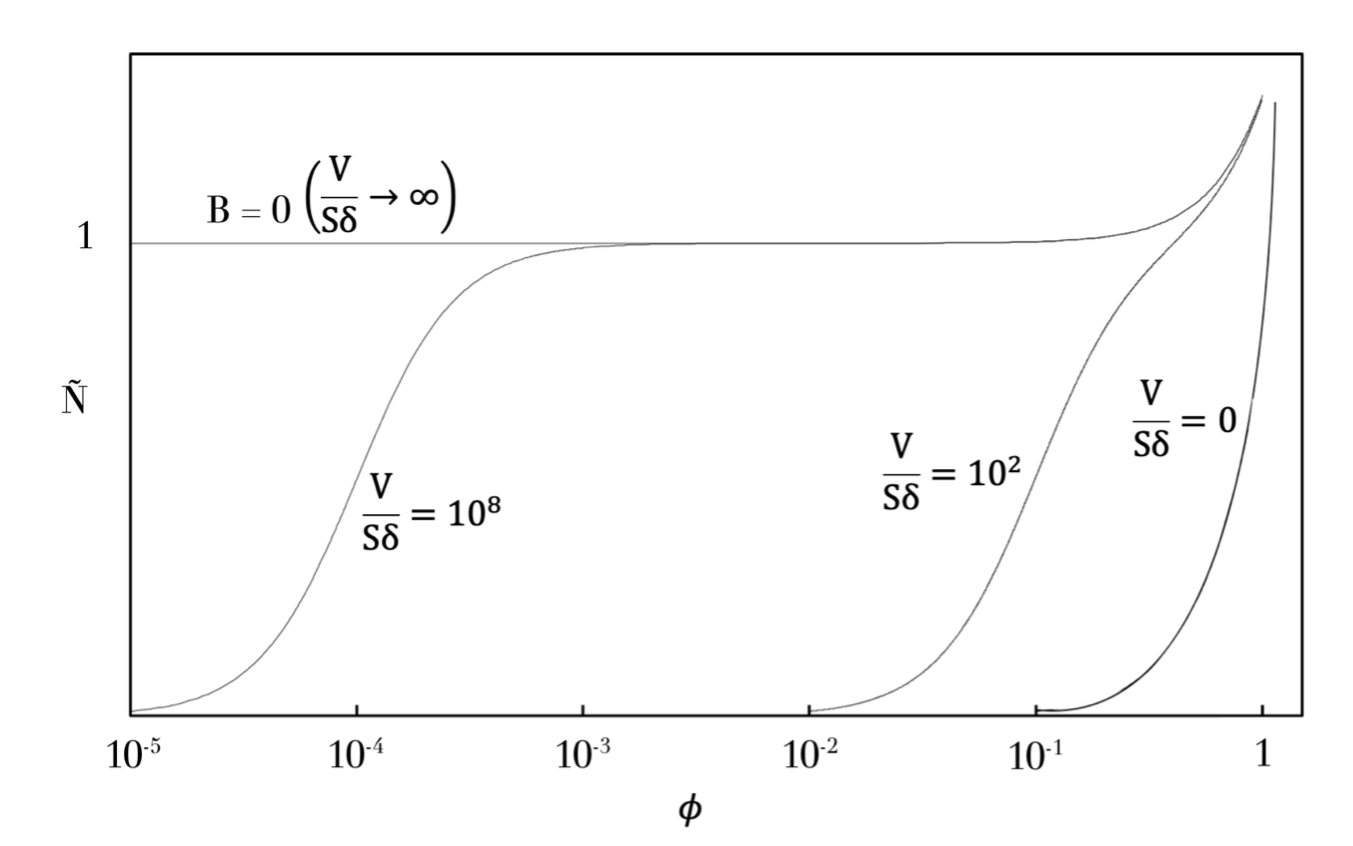
\includegraphics[width=\linewidth]{Capitulo2/Imagenes/Imagen_11_cap_2.png}
    \caption{Absorición de gas con reacción química}
    \label{fig:fig_2.11}
\end{figure}

La ecuación \eqref{eq_2.70} se grafica en la fig. \eqref{fig:fig_2.11}. Se puede observar en la fig. \eqref{fig:fig_2.11}:
\begin{enumerate}
    \item $\widetilde{N}$ aumenta con $\phi$ para todo $\frac{V}{S\delta}$
    \item $\widetilde{N}=1$ es la curva sin reacción que corresponde a la \eqref{fig:fig_2.10}. Cuando $\phi=0$ $\widetilde{N}\rightarrow1$ ($B=0$)
    \item Cuando $\phi\rightarrow0$, para $\frac{V}{S\delta}$ finito $\widetilde{N}=0$, se lidia con un líquido saturado con gas disuelto.
    \item Si $\phi$ es grande, $\widetilde{N}$ se incrementa abruptamente $(B\rightarrow 0)$ y la ec \eqref{eq_2.70} revela que $\widetilde{N}$ es proporcional a $\phi$. La reacción es muy rápida y el gas disuelto se consume dentro de la película. 
    \item Para valores intermedios de $\frac{V}{S\delta}$ y $\phi$, $\widetilde{N}\rightarrow1$. La reacción es rápida y la solución se encuentra libre de soluto. 

\end{enumerate}

\section{Difusión con reacción química heterogénea}

Considérese un reactor catalítico, en donde se lleva a cabo la reacción $2A\rightarrow B$, de acuerdo a la figura \eqref{fig:fig_2.12}

\begin{figure}[H]
    \centering
    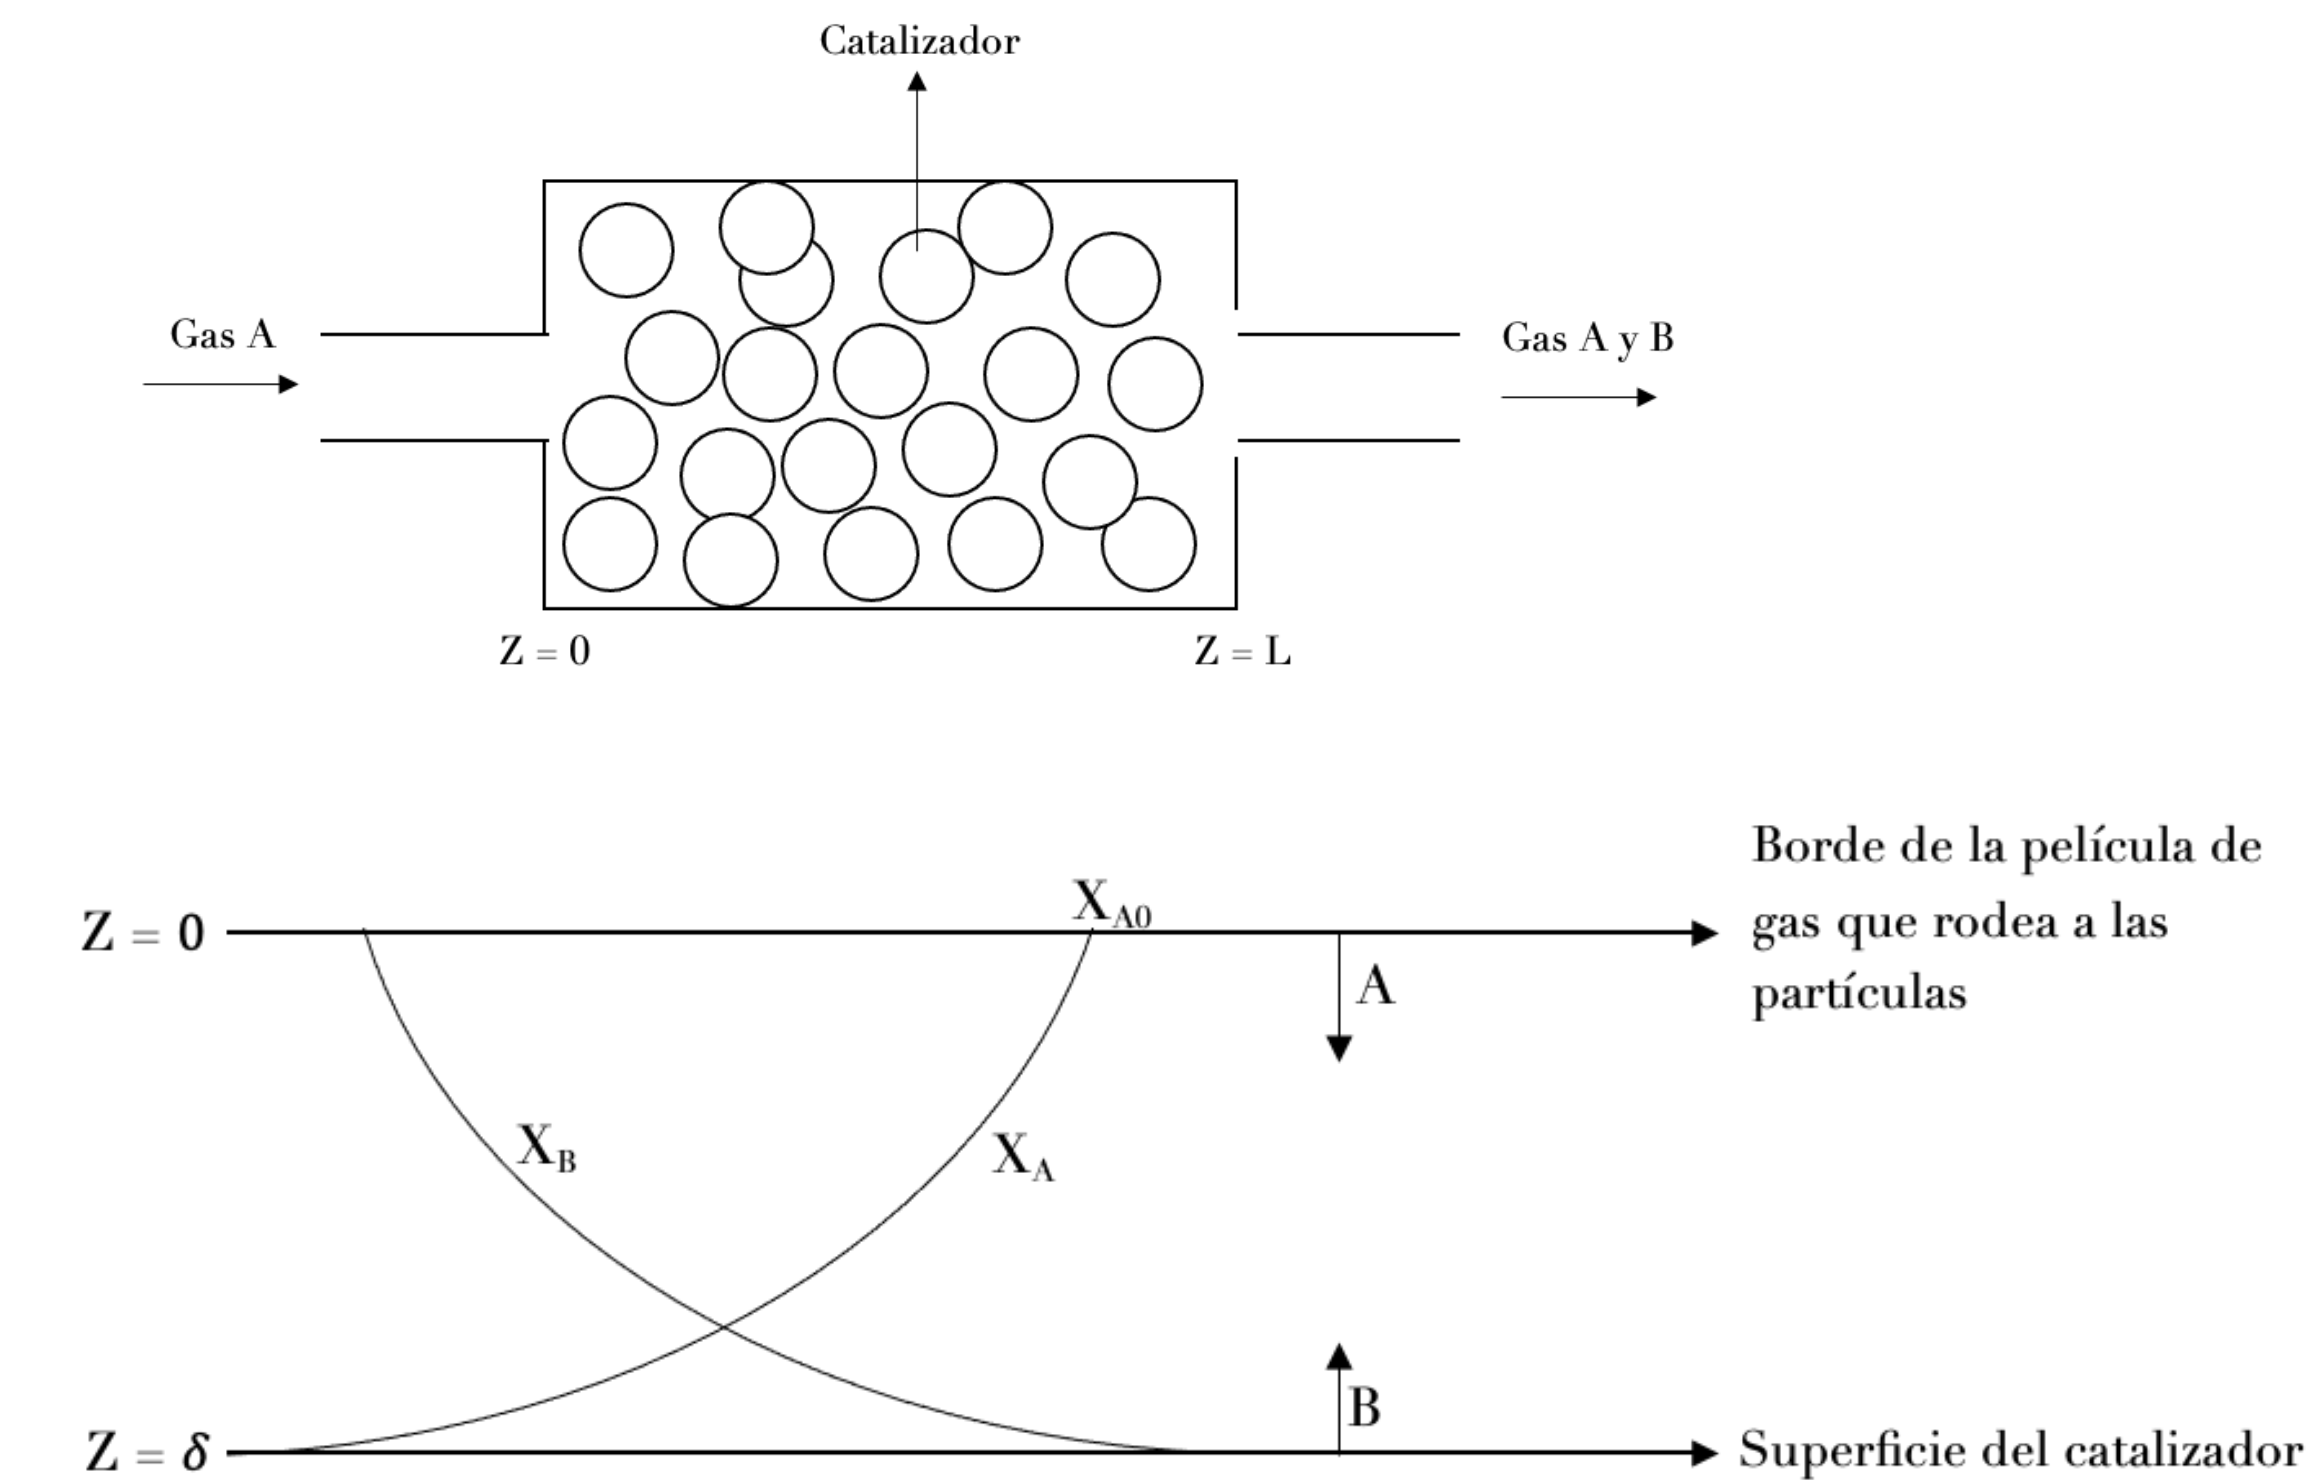
\includegraphics[width=\linewidth]{Capitulo2/Imagenes/Fig_2.12.png}
    \caption{Reactor catalítico en donde $2A\to B$\\Modelo de difusión cerca de la partícula de catalizador}
    \label{fig:fig_2.12}
\end{figure}

2 moles de A se mueven en dirección +z y un mol de B se mueve en dirección -z. Por lo tanto, a régimen permanente:

\begin{equation}
    N_{Bz}=-\frac{1}{2}N_{Az}
    \label{eq_2.71}
\end{equation}

Las ecs \eqref{eq_1.25} y \eqref{eq_1.19} en combinación con la ec \eqref{eq_2.71} son:

\begin{equation}
    N_{Az}=-\frac{c\mathscr{D}_{AB}}{1-\frac{x_A}{2}}\frac{d(x_A)}{dz}
\end{equation}
\begin{equation}
   \text{y} \quad \frac{d(N_A)}{dz}=0
\end{equation}


que resulta en:
\begin{equation}
    \frac{d}{dz}\left(\frac{1}{1-\frac{1}{2}x_A}\frac{dx_A}{dz}\right)=0
    \label{eq_2.74}
\end{equation}




Con las condiciones en la frontera:

\begin{equation}
    x_A |_{z=0} = x_{A0}\quad \text{y} \quad x_A |_{z=\delta} = 0
    \label{eq_2.75}
\end{equation}

A partir de la ec. \eqref{eq_2.74}, se obtiene:

\begin{equation*}
    \frac{1}{1-\frac{x_A}{2}}\frac{dx_A}{dz}=C_1\longrightarrow \int\frac{dx_A}{1-\frac{x_A}{2}}=C_1\int dz +C_2
\end{equation*}

Evaluando $C_1$ y $C_2$ con respecto a las condiciones \eqref{eq_2.75}, se obtiene:

\begin{equation}
    N_{Az}=\frac{2C\mathscr{D}_{AB}}{\delta}\ln\left(\frac{1}{1-\frac{1}{2}x_{A0}}\right)
    \label{eq_2.76}
\end{equation}

La reacción ocurre instantáneamente, por lo que la convección de A en B es un proceso controlado por difusión.

\subsection{Difusión con reacción heterogénea lenta}

En este caso, para el mismo sistema, la reacción no sucede instantáneamente en $z=\delta$, sino que la desaparición de A en la superficie del catalizador es proporcional a la concentración de A en la interfase:

\begin{equation}
    N_{Az}=k_1C_A=k_1Cx_A
\end{equation}

En este caso, la condición de frontera en la superficie del catalizador es:

\begin{equation*}
    x_A|_{z=\delta}=\frac{N_{Az}}{k_1c}
\end{equation*}

El cambio en la condición de frontera, resulta en el siguiente perfil:

\begin{equation}
    \frac{1-\frac{x_A}{2}}{(1-\frac{x_{A0}}{2})^{1-\frac{z}{\delta}}}=\left(1-\frac{N_{Az}}{2k_1c}\right)^{\frac{z}{\delta}}
\end{equation}



\begin{equation}
\begin{split}
     \frac{d}{dz}\ln\left(1-\frac{x_A}{2}\right)-\frac{d}{dz}\left[\left(1-\frac{z}{\delta}\right)\ln\left(1-\frac{x_{A0}}{2}\right)\right]=\frac{d}{dz}\left[\frac{z}{\delta}\ln \left(1-\frac{N_{Az}}{2k_1c}\right)\right]\\-\frac{\frac{1}{2}}{1-\frac{x_A}{2}}\frac{dx_A}{dz}+\frac{1}{\delta}\ln \left(1-\frac{x_{A0}}{2}\right)=\frac{1}{\delta}\ln \left(1-\frac{N_{Az}}{2k_1c}\right)   
\end{split}
\label{eq_2.79}
\end{equation}

Substituyendo la ec \eqref{eq_2.79} en la ec \eqref{eq_2.74}, se obtiene:

\begin{equation*}
    N_{Az}=-\frac{c\mathscr{D}_{AB}}{(1-\frac{x_A}{2})}\left[\left(1-\frac{x_A}{2}\right)\left(\frac{-2}{\delta}\right)\ln \left(\frac{1-\frac{N_{Az}}{k_1c}}{1-\frac{x_{A0}}{2}}\right)\right]
\end{equation*}
Aproximando $\ln (1-\frac{N_{Az}}{2k_1c})\approx -\frac{1}{2}\frac{N_{Az}}{k_1c}$, se obtiene:

\begin{equation*}
   N_{Az}=\frac{2C\mathscr{D}_{AB}}{\delta}\left[-\frac{N_{Az}}{2k_1c}-\ln \left(1-\frac{x_{A0}}{2}\right)\right] 
\end{equation*}
\begin{equation*}
   N_{Az}\left(1+\frac{\mathscr{D}_{AB}}{k_1\delta}\right)=2C\frac{\mathscr{D}_{AB}}{\delta}\ln \left(\frac{1}{1-\frac{1}{2}x_{A0}}\right)  
\end{equation*}
\begin{equation}
   N_{Az}=2c\frac{\mathscr{D}_{AB}}{\delta(1+\frac{\mathscr{D}_{AB}}{k_1\delta})}\ln \left(\frac{1}{1-\frac{1}{2}x_{A0}}\right)  
\end{equation}

El número adimensional $\frac{k_1\delta}{\mathscr{D}_{AB}}=Da$ es el número de Damköler, el cual describe la relación entre reacción y difusión. Si $Da\rightarrow\infty$, se obtiene el caso de reacción dominante y la ecuación toma la forma de la ec. \eqref{eq_2.76}

\section{Difusión con reacción química en medios porosos}

En este caso, se describe la difusión de los reactivos en un medio poroso en términos de una difusividad efectiva ($D_A$). Supóngase que la reacción tiene lugar en la superficie sólida de un catalizador cuya simetría es esférica y posee un radio R, la reacción es $A\rightarrow B$. Esta partícula esférica está sumergida en una corriente de gas con A y B presentes. A se difunde en los poros de la superficie esférica y ahí sucede la reacción. La ec \eqref{eq_1.30} dentro del medio poroso en coordenadas esfericas es:

\begin{equation}
    0=D_A\frac{1}{r^2}\frac{d}{dr}(r^2\frac{d(C_A)}{dr})-R_A
    \label{eq_2.81}
\end{equation}

"a" se define como la superficie catalítica por unidad de volumen (sólido + huecos). Por ello, $R_A=-k_1ac_a$.

Haciendo un cambio de variable, $\frac{C_A}{C_{AR}}=\frac{f(r)}{r}$ en donde $C_{AR}$ es la concentración de A en la superficie esférica, la ec \eqref{eq_2.81} se transforma en:

\begin{equation}
    \frac{d^2f}{dr^2}-\frac{k_1a}{D_A}f=0
    \label{eq_2.82}
\end{equation}

Con condiciones en la frontera:

\begin{equation}
    C_A|_{r=R}=C_{AR} \quad \text{y} \quad C_A|_{r=0}=finito
\end{equation}
o bien:
\begin{equation*}
    f|_{r=R}=R\quad \text{y} \quad
    f|_{r=0}=\text{finito}
\end{equation*}

La solución a la ecuación \eqref{eq_2.82} corresponde a:

\begin{equation}
    f(r)=C_1\cosh[(\frac{k_1a}{D_A})^\frac{1}{2}r]+C_2\sinh[(\frac{k_1a}{D_A})^\frac{1}{2}r]
\end{equation}
\begin{equation*}
    f(0)=C_1=0
\end{equation*}
\begin{equation*}
    f(R)=C_2\sinh[(\frac{k_1a}{D_A})^\frac{1}{2}R]=R\longrightarrow C_2=\frac{R}{sinh[(\frac{k_1a}{D_A})^\frac{1}{2}R]}
\end{equation*}

Por lo tanto:

\begin{equation}
    f(r)=\frac{R\sinh[(\frac{k_1a}{D_A})^\frac{1}{2}r]}{\sinh[(\frac{k_1a}{D_A})^\frac{1}{2}R]}
\end{equation}

Definiendo el modulo de Thiele como $\phi=\sqrt{\frac{k_1a}{D_A}}R$, entonces:
    $f(r)=\frac{R\sinh[\phi(\frac{r}{R})]}{\sinh\phi}$
Luego, 
\begin{equation}
    \frac{C_A}{C_{AR}}=\frac{R}{r}\frac{\sinh[\phi(\frac{r}{R})]}{\sinh\phi}
\end{equation}


Claramente, $\frac{C_A}{C_{AR}}|_{r=0}=\frac{\phi}{\sinh\phi}$ 
\newline
El flujo molar en la superficie es: $W_{AR}=4\pi R^2N_{AR}=-4\pi R^2D_A\frac{d(C_A)}{dr}|_{r=R}$
\begin{equation*}
\begin{split}
        \frac{d(C_A)}{dr}|_{r=R}=\frac{C_{AR}R}{\sinh \phi}\left[\frac{r}{r^2}\cosh\left[\frac{\phi r}{R}\right]\left(\frac{\phi}{R}\right)-\frac{1}{r^2}\sinh \left[\frac{\phi r}{R}\right]\right]\\
=\frac{C_{AR}R}{\sinh (\phi)}\left[\frac{\phi}{R^2}\cosh \phi-\frac{\sinh \phi}{R^2}\right]=\frac{C_{AR}}{R}[\phi \coth \phi-1]
\end{split}
\end{equation*}

Por lo tanto:

\begin{equation}
    W_{AR}=4\pi RC_{AR}D_A[1-\phi \coth (\phi)]
    \label{eq_2.87}
\end{equation}

Definiendo al factor de efectividad $\eta$:

\begin{equation}
    \eta=\frac{N_{AR}}{N_{AR0}}
    \label{eq_2.88}
\end{equation}
En donde $N_{AR0}$ es el flujo molar sin efectos difusionales, es decir:

\begin{equation}
    N_{AR0}=\frac{4\pi R^3}{3}a(-k_1C_{AR})
    \label{eq_2.89}
\end{equation}

Sustituyendo las ecs \eqref{eq_2.87} y \eqref{eq_2.89} en la ec \eqref{eq_2.88} resulta en: 

\begin{equation}
    \eta_A=\frac{3}{\phi^2}[\phi \coth (\phi)-1]
    \label{eq_2.90}
\end{equation}

Físicamente, $\eta_A$ es el factor tal que $\eta_AW_{AR0}$ representa la resistencia difusional del proceso. Para partículas no esféricas, el radio $R_{n e}$ se define como:

\begin{equation}
    R_{ne}=3\left(\frac{V_p}{S_p}\right)
\end{equation}

De tal forma que para partículas esféricas: $\frac{V_p}{S_p}=\frac{\frac{4\pi R^3}{3}}{4\pi R^2}=\frac{R}{3}$

En este caso, el valor de conversión absoluto en la reacción corresponde a:
\begin{equation*}
    |W_{AR}|=V_pak_1C_{AR}\eta_A
\end{equation*}
y donde ahora:
\begin{equation}
    \eta_A=\frac{1}{3\Lambda^2}(3\Lambda \coth 3\Lambda-1)
\end{equation} 
y
\begin{equation}
    \Lambda=(\frac{k_1a}{D_A})^{\frac{1}{2}}(\frac{V_p}{S_p})
\end{equation}
Es el modulo de Thiele generalizado. La variación de $\eta_A$ en función de $\Lambda$ se grafica en la fig \eqref{fig:fig_2.13} para diferentes geometrías

\begin{figure}[H]
    \centering
    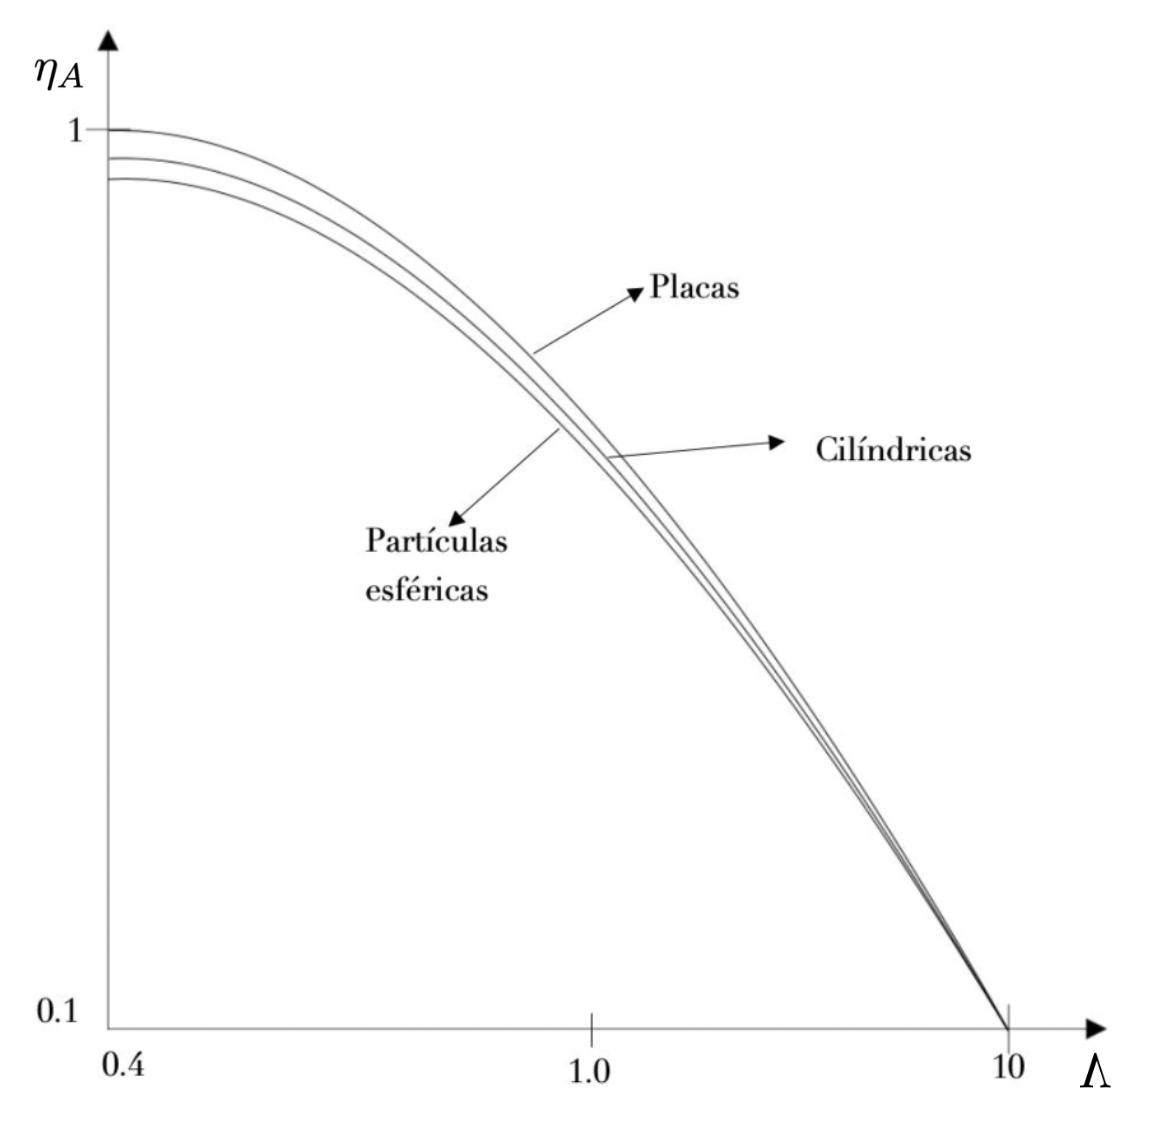
\includegraphics[width=0.7\linewidth]{Capitulo2/Imagenes/Fig_2.13.png}
    \caption{Factores de efectividad en catalizadores porosos de varias fromas}
    \label{fig:fig_2.13}
\end{figure}
\newpage
\section*{Apéndice A}
\begingroup
\renewcommand{\thefigure}{A.\arabic{figure}}
\setcounter{figure}{0}
\renewcommand{\theequation}{A.\arabic{equation}} 
\setcounter{equation}{0}
Difusión debido a una fuente puntual en una corriente de fluído.
Un fluido B fluye a una velocidad constante $v_0$. en algún punto, la especie A se inyecta a un flujo $W_A$ (gmol/s) que es suficientemente pequeño. A se difunde axial y radialmente.

Como este es un problema de convección-difusión, en coordenadas cilíndricas (vea la ec. \eqref{eq_B} en el apéndice B), en la dirección z, se tiene:

\begin{equation}
    \frac{\partial C_A}{\partial t}+v_z\frac{\partial C_A}{\partial z}=\mathscr{D}_{AB}\left[\frac{1}{r}\frac{\partial }{\partial r}\left(r\frac{\partial C_A}{\partial r}\right)+\frac{\partial ^2C_A}{\partial z^2}\right]
\end{equation}
en donde $dt=\frac{dz}{v_0}$.

Ahora, se realiza un cambio de variable $C_A(r,z)=C_A(s,z)$, en la cual $s^2=r^2+z^2$ (ver fig. \eqref{fig:Fig_A.1.})
\begin{figure}[H]
    \centering
    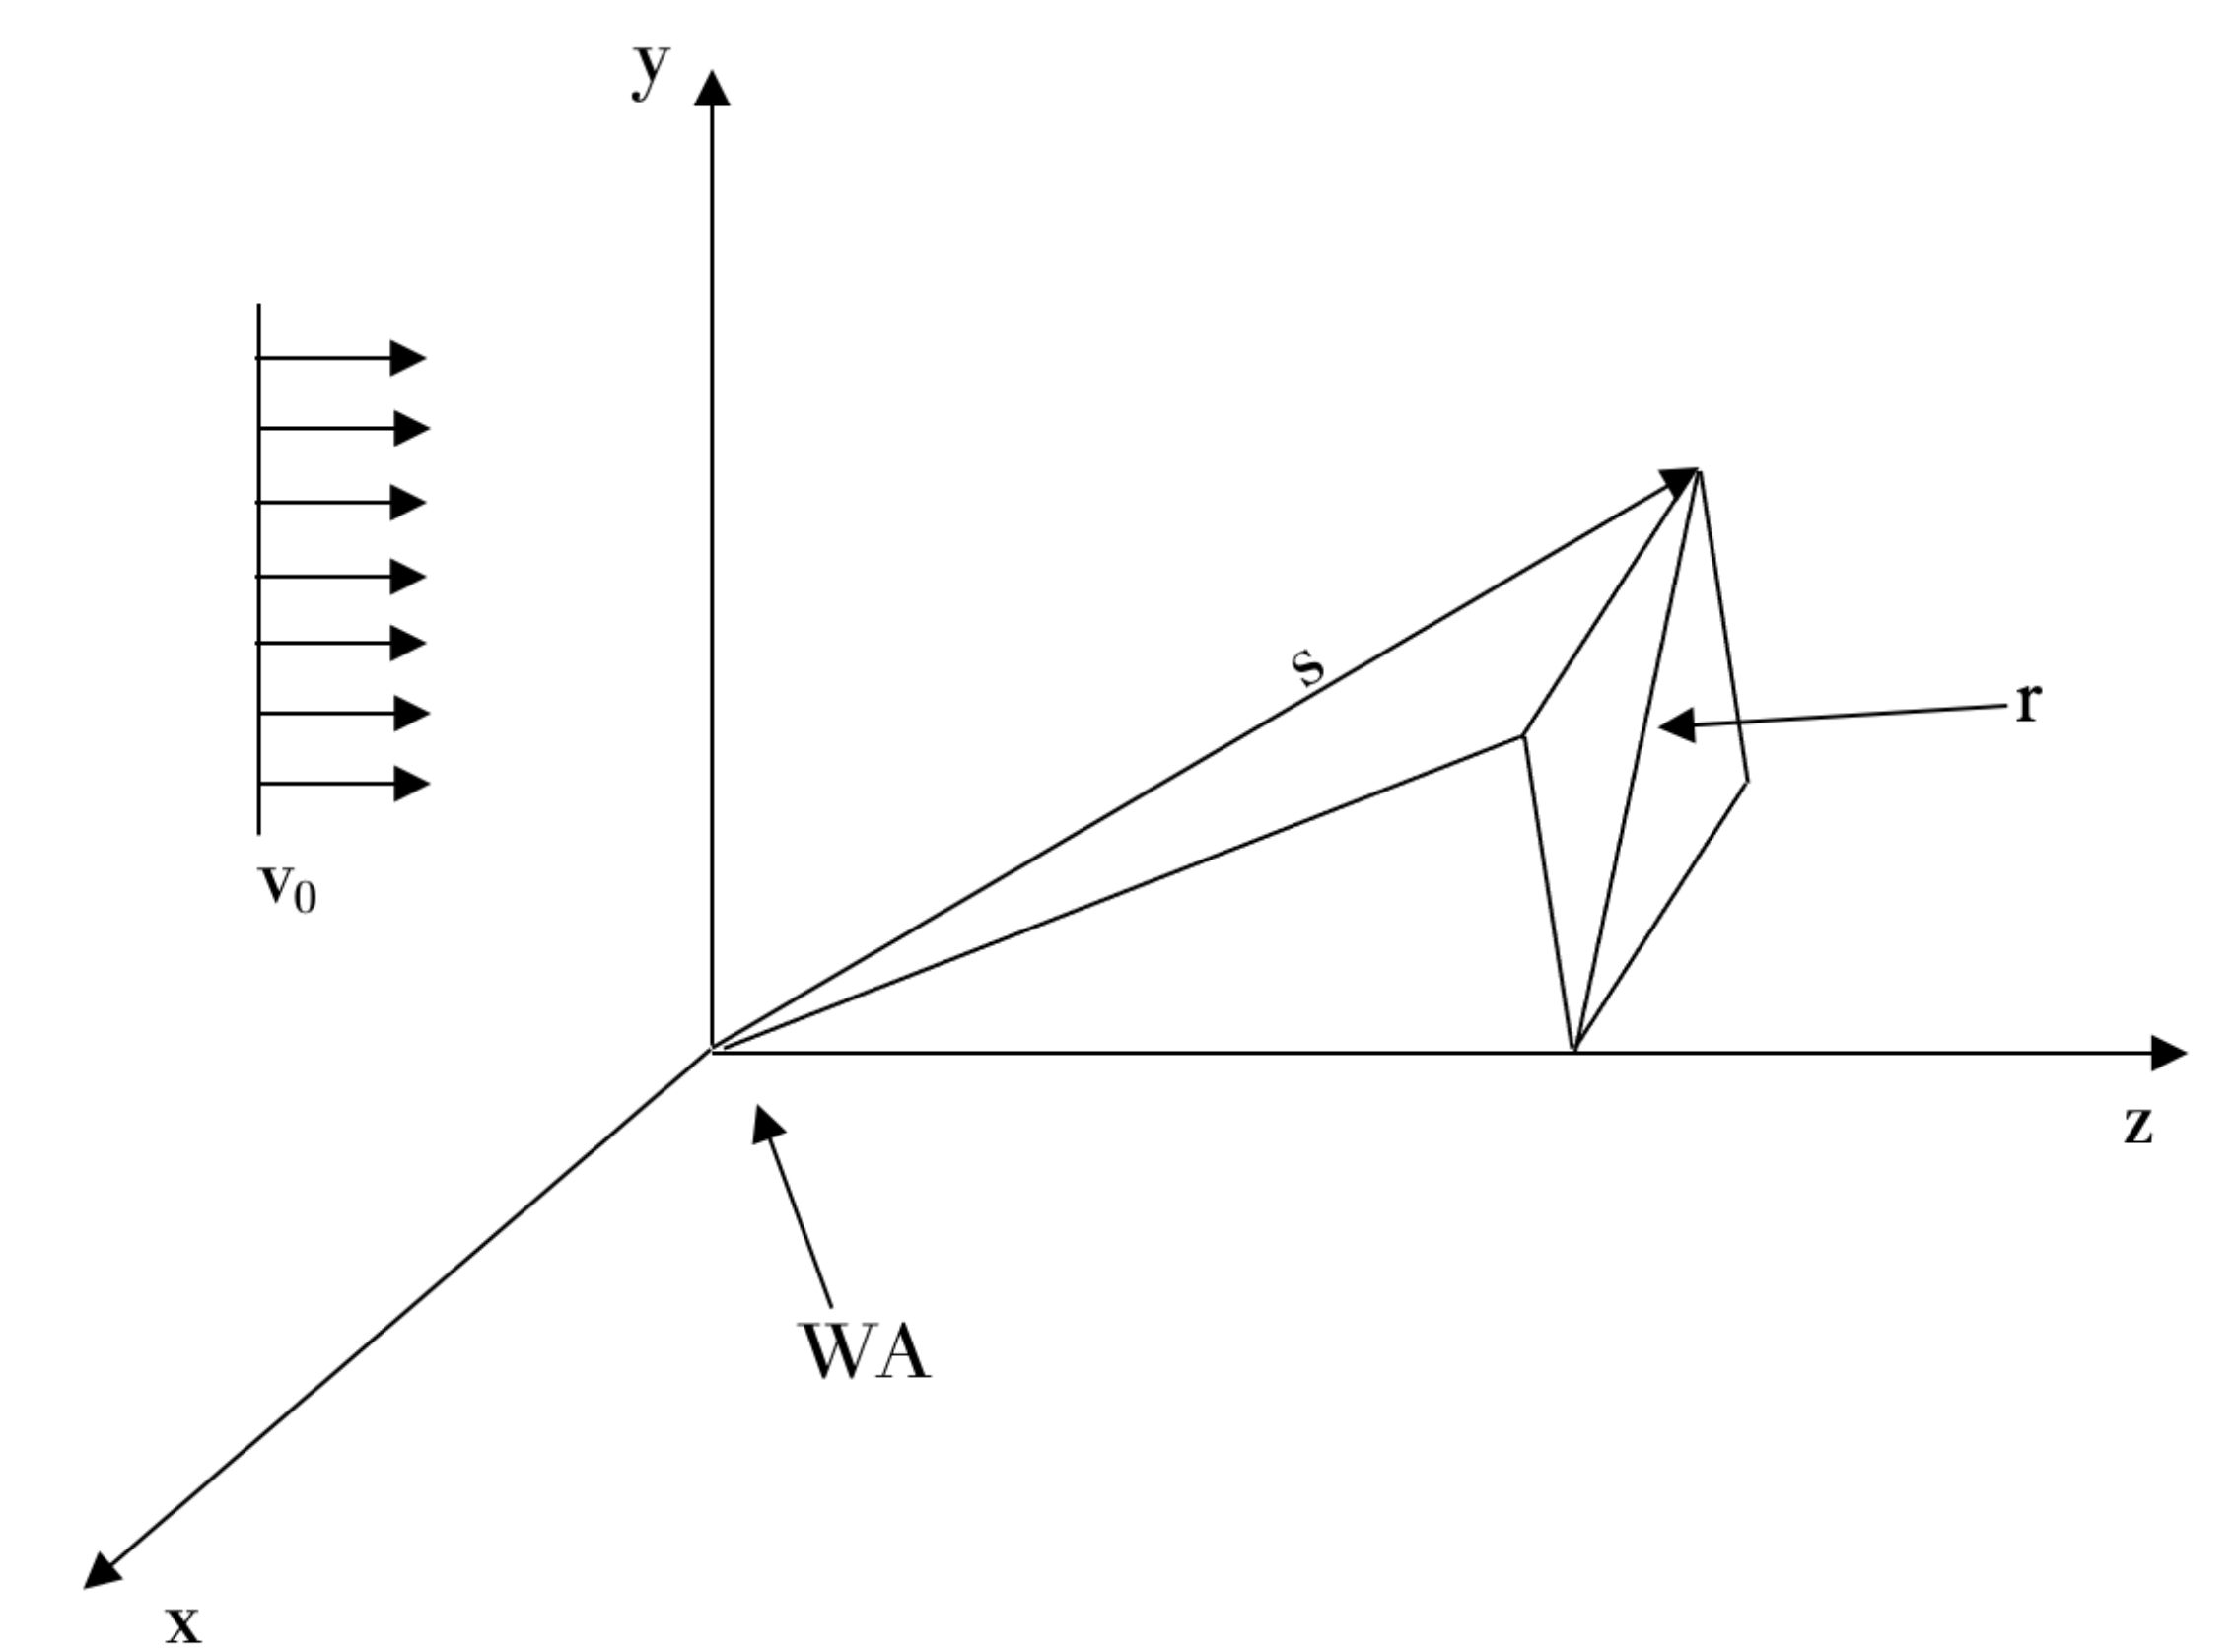
\includegraphics[width=0.5\linewidth]{Capitulo2/Imagenes/Fig_A.1.png}
    \caption{Difusión de A desde una fuente puntual en una corriente de B que va a una velocidad $v_0$ constante}
    \label{fig:Fig_A.1.}
\end{figure}

El diferencial $dC_A$ por regla de la cadena, corresponde a:

\begin{equation*}
    dC_A=(\frac{\partial C_A}{\partial s})_zds+(\frac{\partial C_A}{\partial z})_sdz
\end{equation*}
Luego:
\begin{equation*}
    (\frac{\partial C_A}{\partial z})_r=(\frac{\partial C_A}{\partial s})_z\frac{ds}{dz}+(\frac{\partial C_A}{\partial z})_s
\end{equation*}
Recordando que $s^2=r^2+z^2$, por lo tanto, $\frac{\partial s}{\partial z}=\frac{z}{s}$
\begin{equation*}
    (\frac{\partial C_A}{\partial z})_r=(\frac{\partial C_A}{\partial s})_z\frac{z}{s}+(\frac{\partial C_A}{\partial z})_s
\end{equation*}

\begin{equation*}
    (\frac{\partial^2C_A}{\partial z^2})_r=\frac{\partial}{\partial z}((\frac{dC_A}{dz})_r)
\end{equation*}
\begin{equation*}
    (\frac{\partial^2C_A}{\partial z^2})_r=[\frac{\partial}{\partial s}((\frac{\partial C_A}{\partial s})_r)\frac{\partial s}{\partial z}+\frac{\partial }{\partial z}((\frac{\partial C_A}{\partial s})_r)]_s
\end{equation*}
\begin{equation*}
    (\frac{\partial^2C_A}{\partial z^2})_r=\frac{\partial}{\partial s}[(\frac{\partial C_A}{\partial s})_z\frac{z}{s}+(\frac{\partial C_A}{\partial z})_s]\frac{z}{s}+\frac{\partial }{\partial z}[(\frac{\partial C_A}{\partial s})_z\frac{z}{s}+(\frac{\partial C_A}{\partial z})_s]
\end{equation*}
\begin{equation*}
    (\frac{\partial^2C_A}{\partial z^2})_r=\frac{z}{s}[(\frac{\partial^2 C_A}{\partial s^2})_z\frac{z}{s}-(\frac{\partial C_A}{\partial s})_z\frac{z}{s^2}+\frac{\partial^2C_A}{\partial s \partial z}]
\end{equation*}
\begin{equation*}
    +[(\frac{\partial^2C_A}{\partial z \partial s})\frac{z}{s}+(\frac{\partial C_A}{\partial s})_s\frac{1}{s}+(\frac{\partial^2C_A}{\partial z^2})_s]
\end{equation*}
Se calculan ahora, las derivadas radiales:

\begin{equation*}
    (\frac{\partial C_A}{\partial r})_z=(\frac{\partial C_A}{\partial s})_z(\frac{\partial s}{\partial r})_z=(\frac{\partial C_A}{\partial s})_z(\frac{r}{s})=(\frac{\partial C_A}{\partial s})_z(\frac{(s^2-z^2)^\frac{1}{2}}{s})
\end{equation*}
\begin{equation*}
     r(\frac{\partial C_A}{\partial r})_z=(\frac{\partial C_A}{\partial s})_z(\frac{s^2-z^2}{s})
\end{equation*}
\begin{equation*}
    \frac{1}{r}\frac{\partial}{\partial r}(r(\frac{\partial C_A}{\partial r})_z)=\frac{1}{s}\frac{\partial}{\partial s}[(\frac{s^2-z^2}{s})(\frac{\partial C_A}{\partial s})_z]
\end{equation*}
\begin{equation*}
    =\frac{1}{s}[(\frac{s^2-z^2}{s})(\frac{\partial C_A}{\partial s})_z]+(\frac{s^2-z^2}{s})(\frac{\partial^2C_A}{\partial s^2})_z
\end{equation*}

Sumando, se obtiene:
\begin{equation*}
    \frac{\partial^2C_A}{\partial z^2}+2\frac{z}{s}\frac{\partial^2C_A}{\partial s \partial z}+\frac{\partial^2C_A}{\partial s^2}+\frac{z}{s}(\frac{\partial C_A}{\partial s})
\end{equation*}
O de manera equivalente:
\begin{equation*}
    \frac{\partial^2C_A}{\partial z^2}+2\frac{z}{s}\frac{\partial^2C_A}{\partial s \partial z}+\frac{1}{s^2}\frac{\partial}{\partial s}(s^2\frac{\partial C_A}{\partial s})=f(s,r,z)
\end{equation*}
Al insertar en la ecuación (A.1), se obtiene:
\begin{equation*}
    v_0(\frac{z}{s}\frac{\partial C_A}{\partial s}+\frac{\partial C_A}{\partial z})=\mathscr{D}_{AB}f(s,r,z)
\end{equation*}
Cuya solución es:
\begin{equation}
    C_A=[\frac{W_A}{4\pi \mathscr{D}_{AB}s}]e^{\frac{-v_0(s-z)}{2\mathscr{D}_{AB}}}
\end{equation}
Que satisface las condiciones de frontera:
\begin{equation*}
    1) C_A|_{z \rightarrow \infty}=0 
\end{equation*}
La concentración de A lejos de la fuente es 0
\begin{equation*}
    2) -\frac{\partial C_A}{\partial s}|_{s \rightarrow0}=\frac{W_A}{4\pi \mathscr{D}_{AB}s^2}
\end{equation*}
Este corresponde al sitio de la fuente
\begin{equation*}
    \frac{\partial C_A}{\partial s}=\frac{\partial}{\partial s}[\frac{a}{s}e^{b(s-z)}]=a[\frac{b}{s}e^{b(s-z)}-\frac{1}{s^2}e^{b(s-z)}]=ae^{b(s-z)}[\frac{b}{s}-\frac{1}{s^2}]
\end{equation*}
En donde $a=\frac{W_A}{4\pi \mathscr{D}_{AB}}$, entonces. Si $s\rightarrow 0$, recordando que $s^2=z^2+r^2$, tanto r como z deben tender a 0, por lo tanto:
\begin{equation*}
    \frac{\partial C_A}{\partial s}|_{s\rightarrow 0}=\quad\lim_{s\rightarrow0}ae^{b(s-z)}[\frac{b}{s}-\frac{1}{s^2}]
\end{equation*}
Se toma la siguiente consideración, en el límite $\frac{1}{s^2}>>\frac{b}{s}$ y $e^{b(s-z)=1}$. Por lo tanto:
\begin{equation*}
     \frac{\partial C_A}{\partial s}|_{s\rightarrow 0}=a(-\frac{1}{s^2})
\end{equation*}
y finalmente:
\begin{equation*}
   -\frac{\partial C_A}{\partial s}|_{s\rightarrow 0}=\frac{W_A}{4\pi \mathscr{D}_{AB}s^2} 
\end{equation*}
 \begin{equation*}
     3) \frac{\partial C_A}{\partial r}|_{r\rightarrow0}=0
 \end{equation*}
 Lo cual implica que la concentración máxima está en el eje z
 \begin{equation*}
    \frac{\partial C_A}{\partial r}=\frac{\partial C_A}{\partial s}\frac{\partial s}{\partial r}=\frac{r}{s}\frac{\partial C_A}{\partial s}=\frac{r}{s}(ae^{b(s-z)}[\frac{b}{s}-\frac{1}{s^2}])
 \end{equation*}
 si $r\rightarrow0$, $s\rightarrow z$ y el valor de la derivada es igual a 0, lo que nos dice que el máximo de la función $C_A$ está en el eje z.
 A partir de datos de $v_0$ y $W_A$ dados, se puede plantear un modelo de regresión lineal para la determinación de $\mathscr{D}_{AB}$.
 \begin{equation*}
     ln(C_As)=ln(\frac{W_A}{4\pi \mathscr{D}_{AB}})-v_0\frac{(s-z)}{2\mathscr{D}_{AB}}
 \end{equation*}
 En donde $s-z$ es la variable independiente y $C_{AS}$ la variable dependiente.

\begin{figure}[H]
    \centering
    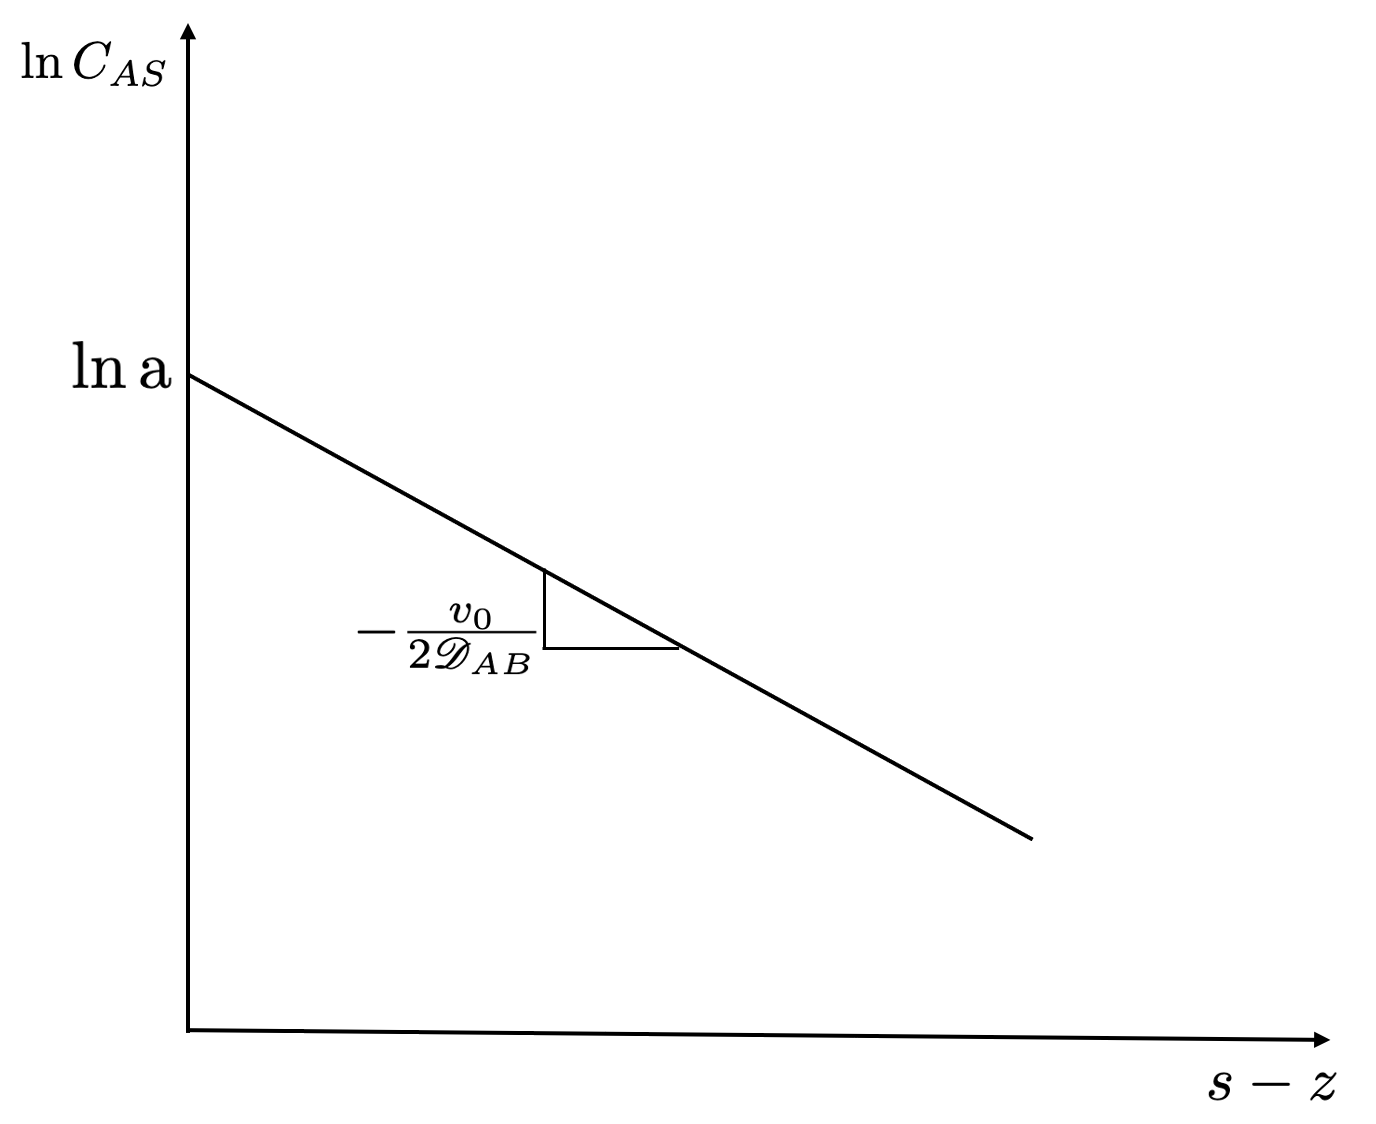
\includegraphics[width=0.5\linewidth]{Capitulo2/Fig_A2.png}
\end{figure}
\endgroup
 


\chapter{Capítulo 3}
Capa Límite con Difusión, Dispersión de Taylor y Flujo Turbulento con Difusión.

Este capítulo consta de las siguientes partes:
\begin{enumerate}
    \item Capa límite.
    \item Convección forzada con reacción química homogéna en una placa plana.
    \item Convección forzada  placa plana con transferencia de masa rápida.
    \item Convección forzada  placa plana con transferencia de masa lenta.
    \item Dispersión de Tayloren flujo laminar.
    \item Transferencia de masa con reacción de $1^{\text{er}}$ orden en flujo laminar turbulento.
    \item Flujo turbulento en reacción de $2^{\circ}$ orden. Mezclado turbulento.
\end{enumerate}
\section{Capa límite binaria}
Considerar un flujo binario a régimen permanente de un fluido binario. En la vecindad de la superficie sólida, las ecuaciones que gobiernan el proceso en ausencia de disipación viscosa son:
 \begin{equation}
\text{Continuidad: }\frac{\partial v_x}{\partial x} + \frac{\partial v_y}{\partial y} = 0 \label{3.1}
\end{equation}
\begin{equation}
    \begin{split}
    \text{Movimiento: } &\rho \left( v_x \frac{\partial v_x}{\partial x} + v_y \frac{\partial v_x}{\partial y} \right) =- \rho v_e \frac{\partial v_e}{\partial x} + \mu \frac{\partial^2 v_x}{\partial y^2} \\
    & + \bar{\rho} g_x \beta (T - T_{\infty}) + \bar{\rho} g_x \bar{\zeta} (w_A - w_{A\infty})
    \end{split}
    \label{3.2}
\end{equation}
\begin{equation}
    \text{Energía: } \rho \bar{C_p} \left( v_x \frac{\partial T}{\partial x} + v_y \frac{\partial T}{\partial y} \right) = 
    k \frac{\partial^2 T}{\partial y^2} - \left( \frac{\bar{H}_A}{M_A} - \frac{\bar{H}_B}{M_B} \right) r_A
    \label{3.3}
\end{equation}
\begin{equation}
    \text{Continuidad de A: } \rho \left( v_x \frac{\partial w_A}{\partial x} + v_y \frac{\partial w_A}{\partial y} \right) = 
    \rho \mathscr{D}_{AB}  \frac{\partial^2 w_A}{\partial y^2} + r_A 
    \label{3.4}
\end{equation}
donde $v_e$ es la velocidad en el límite externo de la capa límite de velocidad, $T_{\infty}$ es la temperatura en el límte externo de la capa límite térmica y $w_{A\infty}$ es la concentración másica en el límite externo de la capa límite difusional.
Los términos de flotación en la ec.(\eqref{3.2}) provenien del efecto témrico y del de concentración. En la ec.\eqref{3.3} se incluye el término de fuente de calor por reacción química. Las ecs.\eqref{3.1}-\eqref{3.4} pueden ser integrados para dar

Ecs. continuidad+movimiento:
\begin{equation}
    \begin{split}
    \mu \frac{du_x}{dy} \bigg|_{y=0} = &\frac{d}{dx} \int_{0}^{\infty} \rho v_x (v_e - v_x) dy + \frac{d v_e}{dx} \int_{0}^{\infty} \rho (v_e - u_x) dy + \rho v_o v_e + \\
   &- \int_{0}^{\infty} \rho g_x \beta (T - T_{\infty}) dy  - \int_{0}^{\infty} \rho g_x \bar{\zeta} (w_A - w_{A\infty}) dy
    \label{3.5}
\end{split}
\end{equation}

Ecs. continuidad+energía:
\begin{equation}
    k \frac{dT}{dy} \bigg|_{y=0} = \frac{d}{dx} \int_{0}^{\infty} \rho v_x \bar{C_p} (T_{\infty} - T) dy
    - \int_{0}^{\infty} \left( \frac{\bar{H}_A}{M_A} - \frac{\bar{H}_B}{M_B} \right) r_A dy
    - \rho v_{\infty} \bar{C_p} (T_{\infty} - T_0) 
    \label{3.6}
\end{equation}

Ecs. continuidad+continuidad de A:
\begin{equation}
    \rho \mathscr {D}_{AB} \frac{dw_A}{dy} \bigg|_{y=0} = \frac{d}{dx} \int_{0}^{\infty} \rho u_x (w_{A\infty} - w_A) dy
    + \int_{0}^{\infty} r_A dy - \rho v_{0} (w_{A\infty} - w_{A0})
    \label{3.7}
\end{equation}

Estas ecuaciones son extensiones de los balances de von Kármán y de la integral de momentum expuestas en el libro 1, Cap. 5.

\section{Convección forzada con reacción química homogénea en una placa plana}
\section{Convección forzada en placa plana con transferencia de masa rápida}
\section{Convección forzada en placa plana con transferencia de masa lenta}
\section{Difusión de Taylor en flujo laminar}
\section{Transferencia de masa con reacción de $1^{er}$ orden en flujo turbulento}


\section{Flujo Turbulento con Reacción de Segundo Orden. Mezclado Turbulento}

Considerar dos casos en los que existen dos solutos $A$ y $B$ disueltos en un solvente $S$. En el primer caso no existe reacción, y en el segundo caso se produce la reacción:
\begin{equation*}
    A + B \rightarrow \text{productos}
\end{equation*}
En ambos casos se estudia el mezclado turbulento en dos sistemas: mezclador estático (a) y dinámico (b).

\begin{figure}[h]

        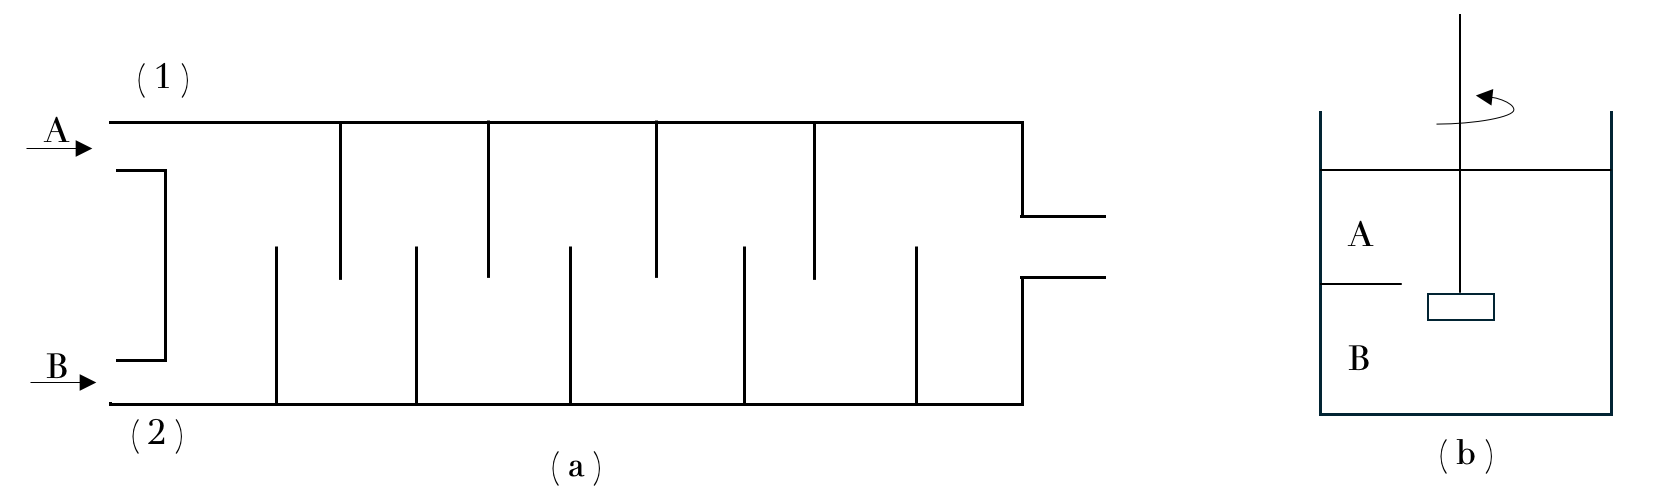
\includegraphics[width=\linewidth]{Capitulo3/Imagenes/Fig_3.8.png}
        \caption{Mezclador estático (a) y mezclador dinámico (b)}
        \label{fig:Fig_3.8}

\end{figure}
        El comportamiento de los solutos A y B se describe por medio de las siguientes ecuaciones de difusión:




\begin{equation}
    \frac{\partial C_A}{\partial t} + \underline{v} \cdot \nabla C_A = \mathscr{D}_{AS} \nabla^2 C_A + R_A
    \notag
\end{equation}

\begin{equation}
    \frac{\partial C_B}{\partial t} + \underline{v} \cdot \nabla C_B = \mathscr{D}_{BS} \nabla^2 C_B + R_B
    \label{eq_3.82}
\end{equation}




Condiciones de frontera:

\begin{equation}
    C_A = C_{A0}, \quad C_B = 0 \quad \text{para } z=0, t=0
    \notag
\end{equation}

\begin{equation}
    C_B = C_{B0}, \quad C_A = 0 \quad \text{para } z=0, t=0
\end{equation}

\subsection{Sin Reacción}

Definiendo:
\begin{equation}
    \Gamma = \frac{C_{A0} - C_A}{C_{A0}} = \frac{C_B}{C_{B0}}
\end{equation}

Las ecuaciones \eqref{eq_3.82} se reducen a:

\begin{equation}
    \frac{\partial \Gamma}{\partial t} + v \cdot \nabla \Gamma = D_{is} \nabla^2 \Gamma
\end{equation}

En las entradas (1) y (2):

\begin{equation}
    \Gamma_1 = 0, \quad \Gamma_2 = 1 \notag
\end{equation}

En flujo turbulento se propone que:

\begin{equation}
    \Gamma = \bar{\Gamma} + \Gamma'
\end{equation}

donde:
\begin{equation}
   \bar{\Gamma} = \frac{C_{A0} - \bar{C}_A}{C_{A0}} = \frac{\bar{C}_B}{C_{B0}}
\end{equation}




y $\Gamma'$ (grado de ausencia de mezclado). Restando $\Gamma$ - $\bar{\Gamma}$  y efectuando el cuadrático medio:

\begin{equation}
    \left( \frac{C_A}{C_{A0}} \right)^2 - \left( \frac{\bar{C}_B}{C_{B0}} \right)^2 = d^2
\end{equation}

En donde $d^2$ es la función de decaimiento que tiende a cero a distancias $z$ grandes o tiempos largos.


La administración de la función de decaimiento indica su dependencia funcional. Definiendo la longitud y velocidades características $l_{0}$ y $v_{0}$, obtuvimos:

\begin{equation}
    \frac{\partial\Gamma}{\partial t} + v_{b}\hat{\nabla}\Gamma = \frac{1}{Re Sc}\hat{\nabla}^{2}\Gamma  \label{eq_3.89}
\end{equation}


donde 

\begin{equation}
      \hat{t}=\frac{v_0t}{l_0}, \quad 
      \hat{v}=\frac{v}{v_0},\quad
      \hat{\nabla}=l_0\nabla, \quad
       Re=\frac{l_0v_0}{\mu}\rho 
\end{equation}

En el caso de tanques de mezclado, $l_0$ es el diámetro del impulson, $v_0=l_0N$ (N es la velocidad angular). En el caso del mezclado de dos corrientes de tubos concéntriccos \eqref{fig:Fig_3.9}, la función de decaimiento resultante se grafica en función de la distnacia axial. El mezclado a nivel molecular (micromezclado) se alcanza

\begin{figure}[h]

        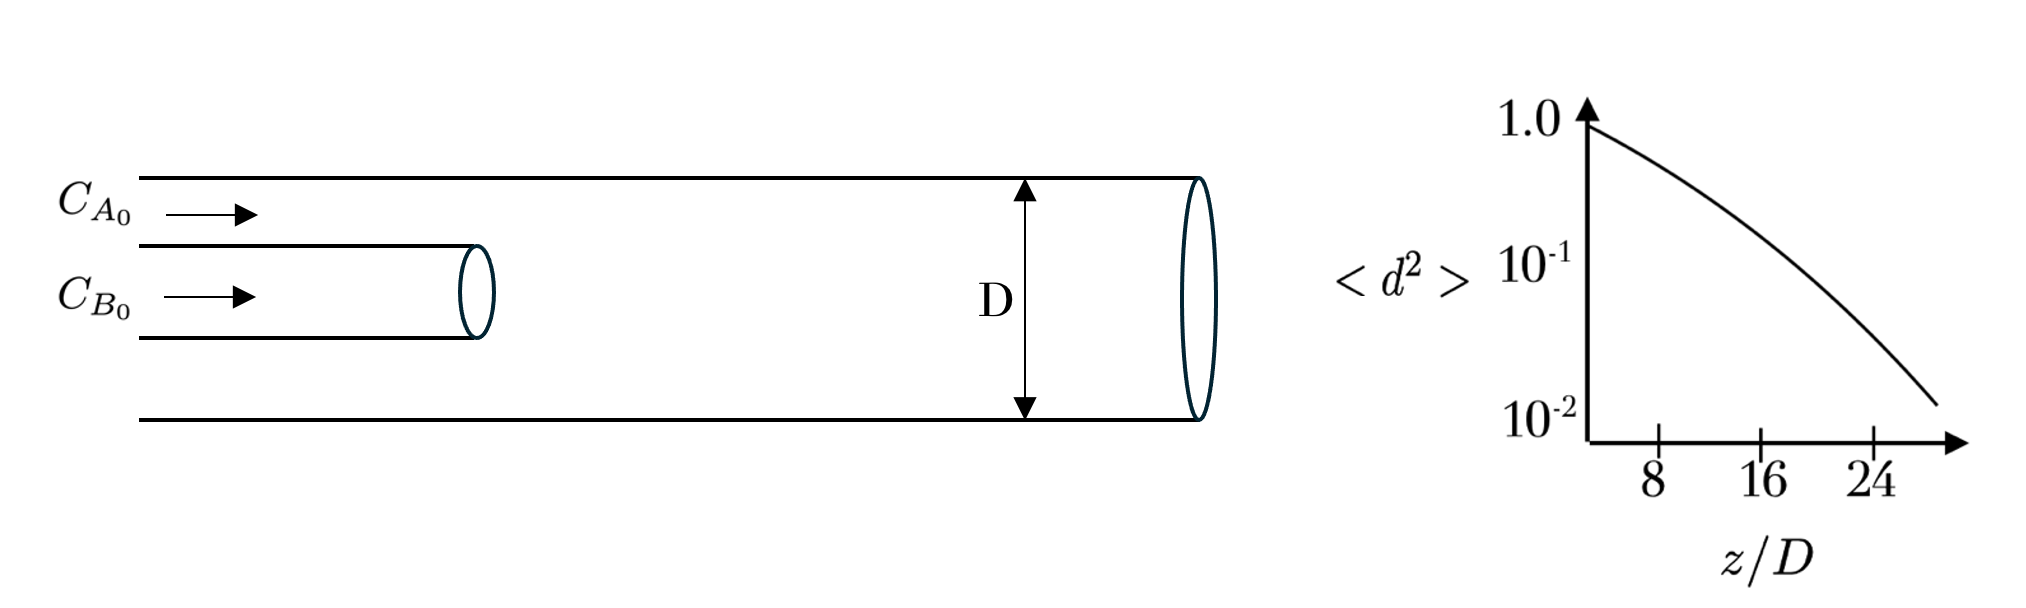
\includegraphics[width=\linewidth]{Capitulo3/Imagenes/Fig_3.9.png}
        \caption{Mezclado de 2 corrientes de A y B en tubos concéntricos y su función de decaimiento}
        \label{fig:Fig_3.9}

\end{figure}

En procesos industriales, normalamente $ReSc\sim10^9$, por lo que la ecuación \eqref{eq_3.89} se reduce a:


\begin{equation}
    \frac{\partial\Gamma}{\partial t} + v_0\hat{\nabla}\Gamma = 0
\end{equation}


Por lo que el grado de mexclado depende de $\hat{t}$ y no de $ReSc$. Como $\hat{t}=Nt_{mix}$, el producto del tiempo de mezclado $t_{mix}$ por la velocidad angular es constante, independiente de $Re$, o sea, $Nt_{mix}=K$, donde K depende de la geometría solamente.

\subsection{Con Reacción}
\begin{equation*}
    A + B \rightarrow \text{productos}
\end{equation*}
Definiendo
\begin{equation}
    \Gamma_{r}=\frac{C_{A0}-(C_A-C_B)}{C_{A0}+C_{B0}}
\end{equation}
Por la resta de las ecuaciones \eqref{eq_3.82}, la descripción del caso con reacción es la misma. Por ello:
\begin{equation}
    \left[ \frac{C_{A0}-(C_A-C_B)}{C_{A0}+C_{B0}} \right]_{reac.}=   \left[ \frac{C_{A0}-C_A}{C_{A0}}\cdot\frac{C_B}{C_{B0}} \right]_{\text{sin reac.} }
\end{equation}
que tambien es válida para las fluctuaciones.
\begin{equation}
        \left[ \frac{C_A'-C_B'}{C_{A0}+C_{B0}} \right]_{reac.}=  \left[ \frac{C_A'}{C_{A0}} \right]_{\text{sin reac.} }
\end{equation}

Esta ecuación sugiere que las fluctuaciones en $C_A$ y $C_B$ en problemas con reacción tienen lugar al mismo tiempo y escalas de distancia que los problemas sin reacción. Los casos particualres son:
\par
a) Reacción rápida: La velocidad de la reacción es controlada por difusión de las especies. Durante la escala del micromezclado, en la que la difusión es lenta en comparación con la convección, el efecto de la reacción es pequeño. En este caso tenemos:
\begin{equation}
            \left( \frac{C_A'}{C_{A0}} \right)_{reac.}=  \left( \frac{C_A'}{C_{A0}} \right)_{\text{sin reac.} }
\end{equation}
En la práctica, las reacciones rápidas son empleadas para determinar la eficiencia de los mezlcados.
\par
b) Reacciones lentas: Considerar el caso de reacciones de segundo orden irreversibles.
\begin{equation}
    R_A=-k_2C_AC_B
\end{equation}
Promediando en el tiempo: 
\begin{equation}
    R_A=-k_(\bar{C_A}\bar{C_B}+C_A'C_B')
\end{equation}
Esto indica que las fluctuaciones en $C_A$ y $C_B$ incrementan la velocidad de reacción. Por medio de un análisis de órdenes de magnitud, tenemos:
\begin{equation}
    t_A=\frac{C_{A0}}{R_A}\sim\frac{1}{k_2C_{B0}}
\end{equation}
Para una reacción rápida $t_{mix}>>t_A$ \newline
Para una reacción lenta $t_{mix}<<t_A$



\newpage
\section* {Apéndice A}
a) Transferencia de masa lenta en una placa plana. Uso de la ecuación \textbf{HACER REFERENCIA A LA ECUACIÓN 3.46}
\newline

Estimación de la velocidad de evaporación, $u_{A0}$, como función de $Sc$, del secado de una placa plana porosa saturada de agua \textbf{HACER REFERENCIA A LA FIGURA 3.2} por medio de una corriente de aire bajo condiciones tal que $W_{A0}=0.05$, $W_{A0}=0.01$ y $Sc=0.6$.
\newline
La ecuación \textbf{HACER REFERENCIA A LA ECUACIÓN 3.46} es:
\begin{equation*}
    \frac{j_{A0}}{\rho v_o(w_{A0}-w_{A\infty})}Sc^{2/3}=0.332\sqrt{\frac{\nu}{v_\infty x}}
\end{equation*}
Por medio de las ecuaciones \eqref{eq_1.24}: $n_{B0}=w_{A_0}(\underline{n}_{A_0}+\underline{n}_{B_0})+\underline{j}_{A_0}$ ya que $\underline{n}_{B_0}=0$, sustituyendo esta ecuación en la \textbf{HACER REFERENCIA A LA EC 3.46}

\begin{equation*}
    \frac{n_{A_0}(1-w_{A_0})}{\rho v_\infty (w_{A_0 }-w_{A\infty)}}=0.332Sc^{-2/3}\sqrt{\frac{\gamma}{v_\infty x}}
\end{equation*}

\begin{equation*}
n_{A_0}=0.332Sc^{-2/3}\frac{(w_{A_0}-w_{A_\infty})}{1-w_{A_0}}\rho v_\infty\sqrt{\frac{\mu}{v_\infty x \rho}}=(0.332)(0.6)^{-2/3}\frac{(0.05-0.01)}{1-0.05}\sqrt{\frac{\rho v_\infty \mu}{x}}
\end{equation*}
\begin{equation*}
    n_{A_0}=0.0196 \sqrt{\frac{\rho v_\infty \mu}{x}}
\end{equation*}
\par
b) Transferencia de momentum, calor y masa simultáneos
\newline
Las ecuaciones \textbf{HACER REFERENCIA A LA EC 3.43} y \textbf{EC 3.44} se pueden generalizar para incluir la transferencia de calor:
\begin{equation}
    \frac{q_0}{\rho \hat{C}pv_\infty(T_0-T_\infty)}=\frac{f''(0)}{Pr}\sqrt{\frac{J}{2v_\infty x}}
    \tag{A-1}
    \label{eq_A-1}
\end{equation}
Las ecuaciones \eqref{eq_A-1}, \textbf{HACER REFERENCIA A LA EC 3.43 3.44} se pueden utilizarse en las transferencias simultáneas generalizando la expresión de k \textbf{HACER REFERENCIA A LA EC 3.38}

\begin{equation}
    K=\frac{\rho_0 v_0 (x)}{\rho v_\infty}\sqrt{\frac{2v_\infty x}{\gamma}}
    \tag{A-2}
    \label{eq_A-2}
\end{equation}
donde $\rho$, $\mu$, $\hat{C}p$ y $\mathscr{D}_{AB}$ sean evaluadas a las condiciones de referencias siguientes: $T_f=\frac{1}{2}(T_0+T_\infty)$ y $W_{Af}=\frac{1}{2}(W_{A_0}+W_{A\infty})$
\newline
La resolución de problemas de transferencia simultáneas se facilita por medio de las siguientes relaciones de los fluxes:

\begin{equation*}
   R_v=\frac{(n_{A_0}+n_{B_0})(v_\infty-e)}{\tau_0} 
\end{equation*}

\begin{equation}
R_T=\frac{(n_{A_0}+n_{B_0})\hat{C}_p(T_o-T\infty)}{q_0} \tag{A-3} \label{eq_A-3}
\end{equation}

\begin{equation*}
R_w=\frac{(w_{A_0}+w_{a_\infty})(n_{A_0}+n_{B_0})}{n_{A_0}-w_{A_0}(n_{A_0}+n_{B_0})}
\end{equation*}

Los R son independientes de x y se relacionan a los números de $\Lambda=(Re,Sc,Pr)$ de acuerdo a:
\begin{equation*}
R=\frac{K\Lambda}{f''(0)} \tag{A-4} \label{eq_A-4}
\end{equation*}
\underline{Ejemplo:} Utilizar las ecuaciones \eqref{eq_A-3} y \eqref{eq_A-4} para obtener ecuaciones implícitas del flux de masa K en la superficie porosa. Para ello, se analizaran 3 casos:

\begin{figure}[h]

        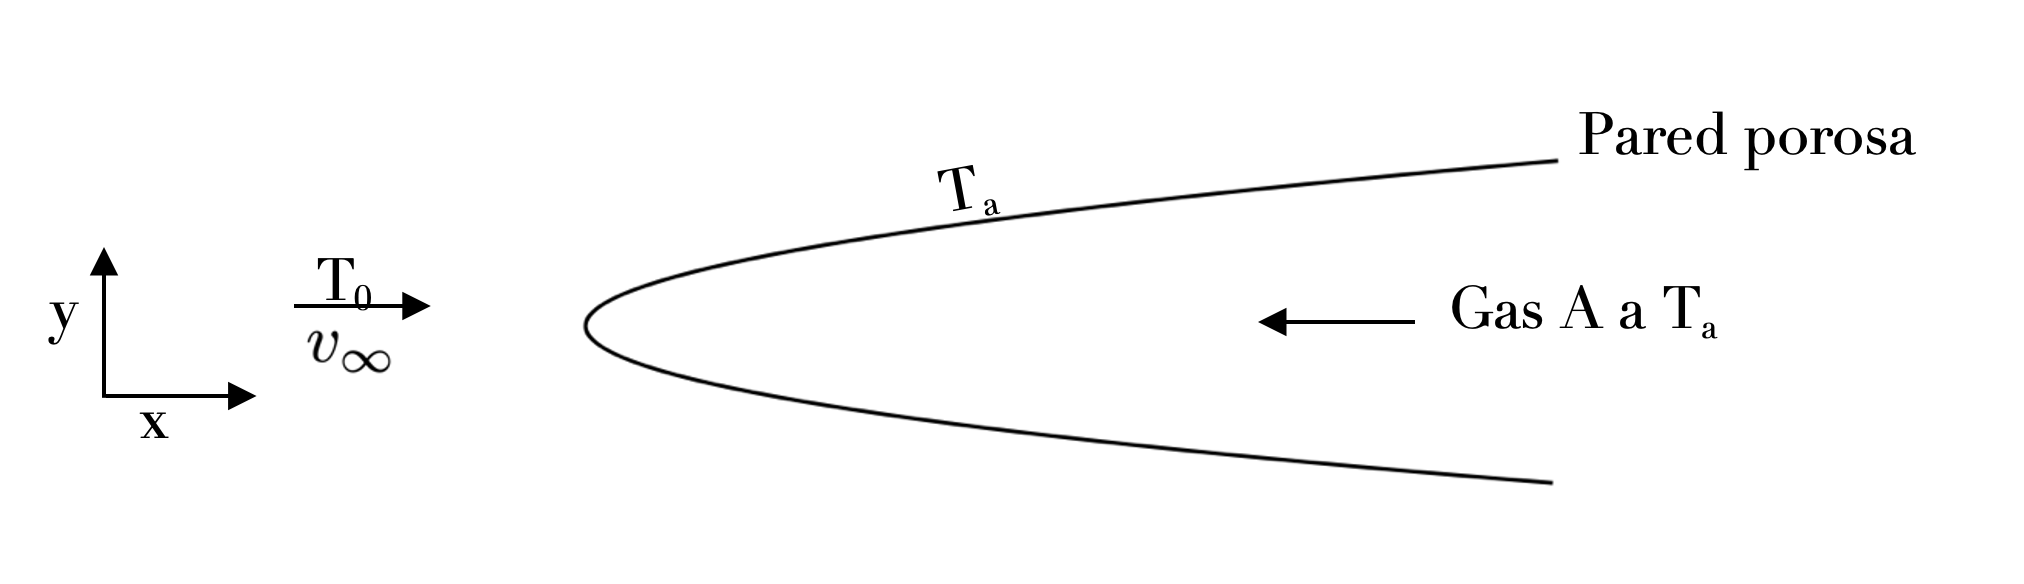
\includegraphics[width=\linewidth]{Capitulo3/Imagenes/Fig_A.1.png}
    \caption{Enfriamiento por transpiración en una placa porosa.}
        \label{fig:Fig_A.1}

\end{figure}

\begin{enumerate}
    \item Evaporación de un líquido A en una corriente de A y B. B es insoluble en A. \newline
    Como $n_{B_0}=0$, $R_w$ en \eqref{eq_A-3} se puede calcular: $R_w=\frac{w_{A_0}-w_{A\infty}}{1-w_{A_0}}$, donde $K=\frac{R_w f''(0)}{Sc}=\frac{1}{Sc}\frac{w_{A_0}-w_{A\infty}}{1-w_{A_0}}f''(0)$
    \item Reacción irreversible de A (gas) en C (sólido) $\to$ B (gas) de acuerdo a $A+C\to 2B$. Pesos moleculares de A y B son iguales. Como $n_{B_0}=-2n_{A_0}$ y $w_A=0$, $R_w=\frac{0-w_{A_\infty}}{-1}=w_{A_\infty}$, donde $K=\frac{1}{Sc}w_{a_\infty f''(0)}$
    \item Enfriamiento por transpiración. Gas A solamente
    \newline 
    Balance de energía:
    \begin{equation*}
        q_0=v_0\hat{C}_p\rho_0(T_a-T_0 )=n_{A_0}\hat{C}_p(T_a-T_0)
    \end{equation*}
    De las ecuaciones \eqref{eq_A-3}: $R_T=\frac{n_{A_0}\hat{C}_p(T_o-T\infty)}{n_{A_0}\hat{C}_p(T_a-T_0)}$
    \newline
    El valor de \( K \) es: \[ K = \frac{1}{Pr} \left( \frac{T_0 - T_\infty}{T_a - T_0} \right) f''(0) \]
\end{enumerate}

\end{document}
